
% Routh-Hurwitz Stability Analyzer LaTeX Paper
\documentclass[11pt]{article}
\usepackage{amsmath,amsfonts,amssymb}
\usepackage{graphicx}
\usepackage{float}
\usepackage{listings}
\usepackage{tikz}
\usepackage{geometry}
\geometry{margin=1in}

\title{Routh-Hurwitz Stability Analyzer: A MATLAB App for Symbolic and Numeric Evaluation of LTI Systems}
\author{Harshit Pranjal \\
Department of Mathematics \\
Birla Institute of Technology, Mesra, Ranchi \\
\texttt{imh1001924@bitmesra.ac.in}}
\date{}

\begin{document}

\maketitle

\begin{abstract}
This paper presents a MATLAB-based application titled \emph{Routh-Hurwitz Stability Analyzer}, designed to analyze the stability of linear time-invariant (LTI) systems using the classical Routh-Hurwitz criterion. The app accepts both symbolic and numeric inputs and automatically generates the corresponding polynomial, constructs the Routh-Hurwitz table, evaluates sign changes, plots system roots, and provides a stability verdict. The application serves as an educational and research verification tool to help reduce human errors in system stability analysis.
\end{abstract}

\section{Introduction}
Stability is a fundamental requirement in control systems. A system is considered stable if its output remains bounded for any bounded input. In many real-world systems — such as power electronics, aerospace control, and biomedical applications — ensuring stability is critical for safe operation.

The Routh-Hurwitz criterion offers an algebraic method for determining whether all roots of a system's characteristic polynomial lie in the left half of the complex plane, without explicitly computing the roots. Its application avoids complex root-solving, especially for high-order systems where analytical solutions are impractical.

Despite its robustness, manual construction of the Routh table is prone to human error, especially when encountering special cases like zero rows or symbolic expressions. To address this challenge, this paper introduces a MATLAB-based application that automates the Routh-Hurwitz procedure. It accepts both symbolic and numeric inputs, evaluates stability, generates graphical root plots, and simplifies the process for learners and researchers alike.

The Routh-Hurwitz method determines the stability of a linear time-invariant (LTI) system by examining the sign variations in the first column of a constructed Routh array derived from the characteristic polynomial. The mathematical formulation eliminates the need for explicitly solving high-degree polynomials, which is particularly useful in control system design where analytical root calculation becomes infeasible.

However, manually constructing the Routh table can be tedious and error-prone, especially when handling zero entries or symbolic expressions. These challenges have led to the demand for reliable computational tools to support students and researchers. Motivated by this need, this paper introduces a MATLAB-based application that automates the Routh-Hurwitz process. The application not only supports both symbolic and numeric analysis but also incorporates stability evaluation, graph plotting, and data export functionalities. It aims to facilitate learning and reduce the probability of human error in mathematical verification and research documentation.

\section{Theoretical Background}
The Routh-Hurwitz criterion determines system stability by analyzing sign changes in the first column of a specially constructed Routh table. For a characteristic polynomial:
\[ P(s) = a_0s^n + a_1s^{n-1} + \ldots + a_n, \]
the number of roots with positive real parts equals the number of sign changes in the first column of the Routh array.The significance of Routh-Hurwitz-based stability analysis in compartmental disease models, particularly SIR-type models, has been demonstrated in earlier studies~\cite{paper2}.

Special handling is required when a zero appears in the first column or when an entire row is zero. The algorithm incorporates auxiliary polynomial methods and small epsilon substitutions to maintain numerical robustness.

The theoretical foundation of the Routh-Hurwitz criterion follows from standard graduate-level control literature, such as the ECE 680 lectures~\cite{ece680}.

\section{App Design and Features}
The \emph{Routh-Hurwitz Stability Analyzer} is built using MATLAB R2025a's App Designer. Key features include:
\begin{itemize}
    \item Symbolic or numeric input modes
    \item Polynomial auto-generation (for both numeric and symbolic inputs)
    \item Routh-Hurwitz table construction
    \item Stability detection with sign change counter
    \item Root plotting on the complex plane (numeric input only)
    \item Downloadable outputs and graph (numeric mode)
    \item Embedded help system for educational support
    \item Note: The app is only valid for algebraic polynomials and does not support transcendental polynomials (e.g., those involving exponential or logarithmic terms).
\end{itemize}

\begin{figure}[H]
    \centering
    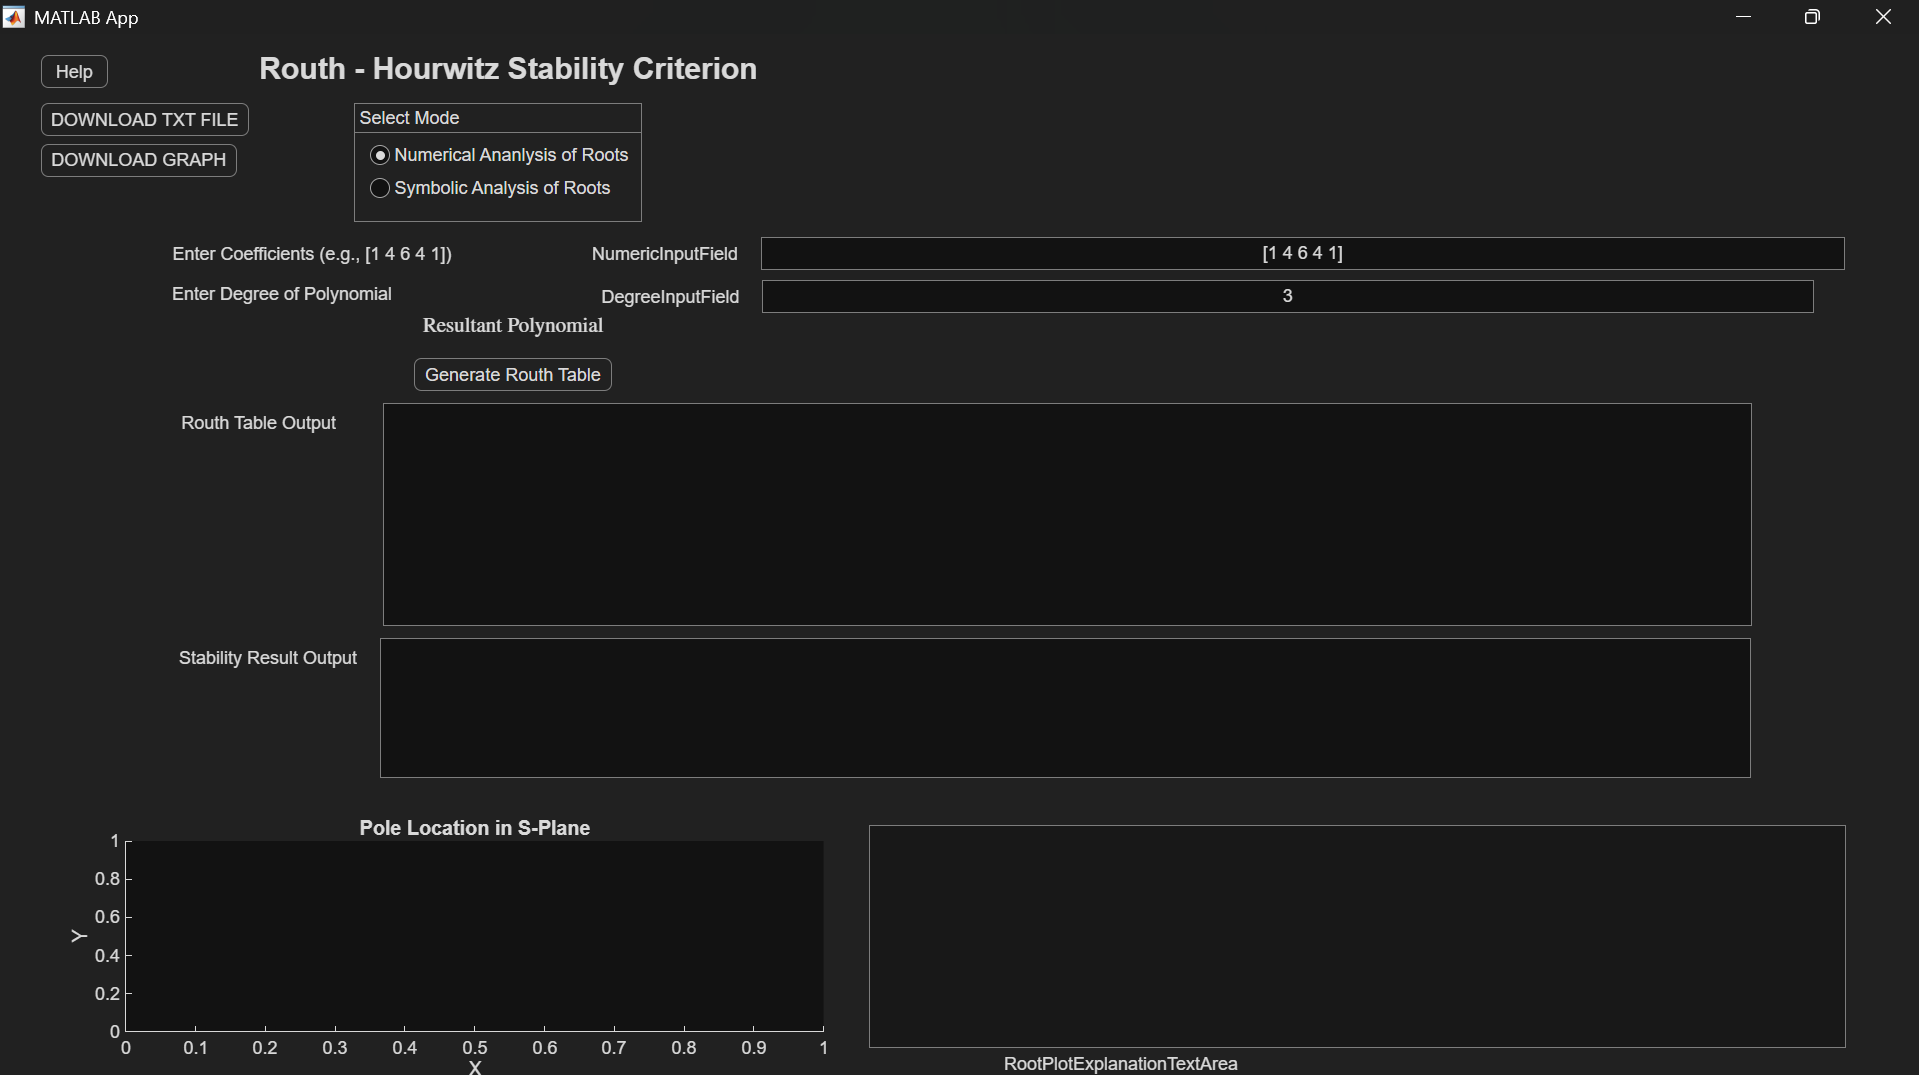
\includegraphics[width=0.5\textwidth]{app_ui.png}
    \caption{Workflow of the Routh-Hurwitz Stability Analyzer app}
\end{figure}
\begin{figure}[H]
    \centering
    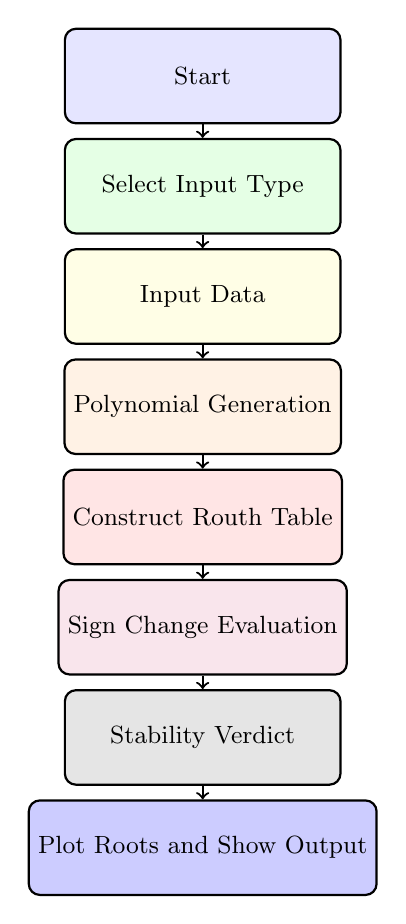
\begin{tikzpicture}[node distance=1.4cm, every node/.style={draw, align=center, rounded corners, minimum width=3.5cm, minimum height=1.2cm, font=\small}, every path/.style={->, thick}]
        \node[fill=blue!10] (start) {Start};
        \node[fill=green!10, below of=start] (mode) {Select Input Type};
        \node[fill=yellow!10, below of=mode] (input) {Input Data};
        \node[fill=orange!10, below of=input] (poly) {Polynomial Generation};
        \node[fill=red!10, below of=poly] (routh) {Construct Routh Table};
        \node[fill=purple!10, below of=routh] (eval) {Sign Change Evaluation};
        \node[fill=gray!20, below of=eval] (verdict) {Stability Verdict};
        \node[fill=blue!20, below of=verdict] (result) {Plot Roots and Show Output};

        \draw (start) -- (mode);
        \draw (mode) -- (input);
        \draw (input) -- (poly);
        \draw (poly) -- (routh);
        \draw (routh) -- (eval);
        \draw (eval) -- (verdict);
        \draw (verdict) -- (result);
    \end{tikzpicture}
    \caption{Simplified vertical flowchart of the Routh-Hurwitz Stability Analyzer app}
\end{figure}

\section{Methodology}
The methodology consists of the numerical construction of the Routh-Hurwitz table from the user’s input, automated handling of special cases, and derivation of the system’s stability conclusion. The core computational logic is encapsulated in the custom MATLAB function \texttt{routhAnalyzer}. This function executes the following steps:

\begin{enumerate}
    \item Accept the input coefficients or degree, depending on mode.
    \item Construct the first two rows of the Routh table from the input.
    \item Fill subsequent rows using the standard Routh-Hurwitz determinant formula.
    \item Implement zero handling logic:
    \begin{itemize}
        \item Replace near-zero entries with epsilon ($\varepsilon = 10^{-6}$) to avoid division by zero.
        \item When an entire row becomes zero, generate the auxiliary polynomial using the row above and differentiate to replace it.
    \end{itemize}
    \item Count sign changes in the first column.
    \item Generate the verdict: Stable (no sign changes) or Unstable (sign changes present).
    \item Plot the roots on the complex plane for graphical validation.
\end{enumerate}

The MATLAB implementation is summarized below:

\begin{lstlisting}[language=Matlab, caption=routhAnalyzer.m -- Core Logic]
function [routhTable, stabilityStatement, signChanges] = routhAnalyzer(coeffs)
% Computes Routh-Hurwitz table and determines system stability
... % Paste your MATLAB code here, trimmed if needed
end
\end{lstlisting}
The core computation for constructing the Routh table and analyzing system stability is implemented in the MATLAB script \texttt{routhAnalyzer.m}, which is responsible for all backend numerical and symbolic evaluations. The graphical user interface (GUI), user input handling, mode selection, result display, and export functionalities are integrated through MATLAB App Designer and bundled as \texttt{RouthStability.mlapp}.

For code access or academic reference, readers may contact the author. Both the logic script and GUI app file are available upon request or may be shared via the institutional repository (if hosted).


This methodology ensures accurate, symbolic-compatible, and robust Routh table construction suitable for educational and research-level control system design.

\section{Case Studies}
\subsection{Numeric Example}
Input: \texttt{[1 4 6 4 1]} \\

\begin{figure}[H]
  \centering
  \begin{minipage}[t]{0.49\textwidth}
    \centering
    \includegraphics[width=\textwidth]{Routhreport.png}
    \caption*{(a) Routh Table Output}
  \end{minipage}
  \hfill
  \begin{minipage}[t]{0.49\textwidth}
    \centering
    \includegraphics[width=\textwidth]{routh_graph.png}
    \caption*{(b) Root Plot}
  \end{minipage}
  \caption{Numeric Input Analysis: Table and Root Plot}
  \label{fig:numeric_results}
\end{figure}

\newpage
\subsection{Numeric Example 2}
Input: \texttt{[1 4 6 5 7 1]} \\

\begin{figure}[H]
  \centering
  \begin{minipage}[t]{0.40\textwidth}
    \centering
    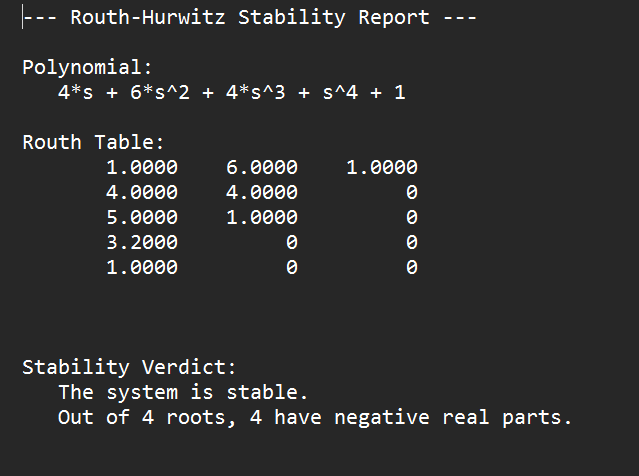
\includegraphics[width=\textwidth]{routh_report1.png}
    \caption*{(a) Routh Table Output}
  \end{minipage}
  \hfill
  \begin{minipage}[t]{0.49\textwidth}
    \centering
    \includegraphics[width=\textwidth]{routh_graph1.png}
    \caption*{(b) Root Plot}
  \end{minipage}
  \caption{Numeric Input Analysis for $[1, 4, 6, 5, 7, 1]$: Table and Root Plot}
  \label{fig:numeric_results_2}
\end{figure}

\subsection{Symbolic Examples}
Input: Degree = 3 and 4 \\

\begin{figure}[H]
  \centering
  \begin{minipage}[t]{0.40\textwidth}
    \centering
    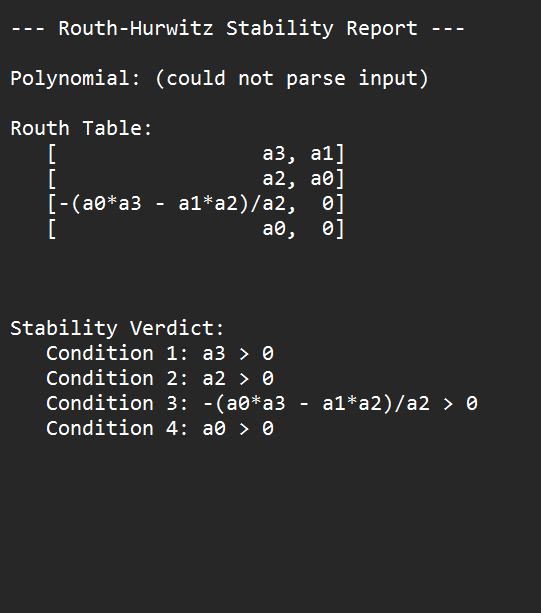
\includegraphics[width=\textwidth]{routh_reportsym.png}
    \caption*{(a) Symbolic Routh Table (Degree = 3)}
  \end{minipage}
  \hfill
  \begin{minipage}[t]{0.40\textwidth}
    \centering
    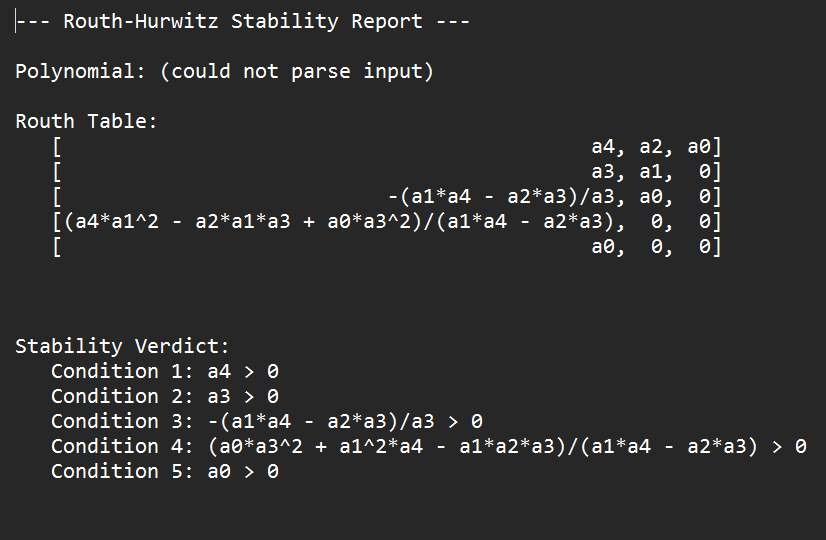
\includegraphics[width=\textwidth]{routh_reportsym1.png}
    \caption*{(b) Symbolic Routh Table (Degree = 4)}
  \end{minipage}
  \caption{Symbolic Evaluation for Degrees 3 and 4}
  \label{fig:symbolic_examples}
\end{figure}

\section{Conclusion and Future Scope}
The presented MATLAB app provides a robust, accessible way to perform Routh-Hurwitz stability analysis. It reduces human error, improves accessibility for new researchers, and enhances learning through symbolic and numeric flexibility.

In future versions, the app can be extended to handle delay differential equations and systems with fractional-order dynamics. Additionally, integration with eigenvalue analysis modules and machine learning tools may enhance its capability in automatic error correction and research verification workflows. Such improvements would broaden its utility from an educational aid to a comprehensive research tool. The proposed system can be extended toward fractional-order dynamic modeling frameworks as seen in recent research on plant disease systems~\cite{paper3}.

\vspace{0.5em}
\noindent
Currently, the application supports stability analysis for algebraic polynomials only. It does not handle transcendental characteristic equations (such as those involving exponential or logarithmic terms), which commonly arise in time-delay or infinite-dimensional systems. The author is actively exploring methods to incorporate such systems into future versions of the app, including extensions toward quasi-polynomials and Laplace domain representations.

\vspace{1em}
\noindent\textbf{Final Remarks.} 
This tool bridges the gap between theoretical Routh-Hurwitz analysis and practical system validation by offering a user-friendly, error-resilient computational interface. It makes research in this field more engaging, visual, and largely error-free — catering even to young researchers who have just stepped into control system theory.

\section*{Author's Note}
The author has independently developed this application and prepared the accompanying analysis, aiming to support fellow researchers and learners working in the domain of system stability.

\section*{References}
\begin{thebibliography}{9}

\bibitem{ogata}
K. Ogata, \textit{Modern Control Engineering}, 5th ed., Prentice Hall, 2010.

\bibitem{matlab}
MATLAB and App Designer, Version R2025a, The MathWorks, Inc., Natick, Massachusetts, United States.

\bibitem{paper1}
P. K. Shaw, “Impact of Vaccination and Treatment in a Fractional SIRV Measles Model: A Comparative Numerical Study,” Manuscript.

\bibitem{paper2}
D. Ezekiel, “Stability Analysis of an SIR Infectious Disease Model,” \textit{International Journal of Nonlinear Science}, vol. 12, no. 2, pp. 107–113, 2011.

\bibitem{paper3}
P. K. Shaw, S. Kumar, S. Momani, and S. Hadid, “Dynamical Analysis of Fractional Plant Disease Model with Curative and Preventive Treatments,” \textit{Chaos, Solitons \& Fractals}, vol. 156, Article ID 111830, 2022.

\bibitem{ece680}
ECE 680 Lecture Notes, “Modern Automatic Control: Routh's Stability Criterion,” Purdue University, 2007.

\end{thebibliography}

\end{document}
